\begin{frame}{\ptthreeofour structure appears with oxygen}
    \begin{columns}
    
    \column[T]{0.38\textwidth}
    \begin{table}
        \centering
        \begin{tabular}{ |l|l|l|l| }
            \hline
            Argon & \ammonia & \dioxygen & Duration \\
             & & & (hours) \\ 
            \hline
            50 & 0 & 0 & 24 \\
            \rowcolor{shadecolor}
            42 & 0 & 8 & 12 \\
            41 & 1 & 8 & 5 \\
            % \hline
            % 50 & 0 & 0 & 7 \\
            % 42 & 0 & 8 & 1 \\
            % 41 & 1 & 8 & 10 \\
            % 48.5 & 1 & 0.5 & 13 \\
            % 49 & 1 & 0 & 11 \\
            % 50 & 0 & 0 & 8 \\
            \hline
        \end{tabular}
        \caption{Gas flow in reactor ($50$ mL/min, $0.3$ bar). In experimental order.}
    \end{table}

    \vspace{-0.5cm}

    \begin{figure}
        \centering
        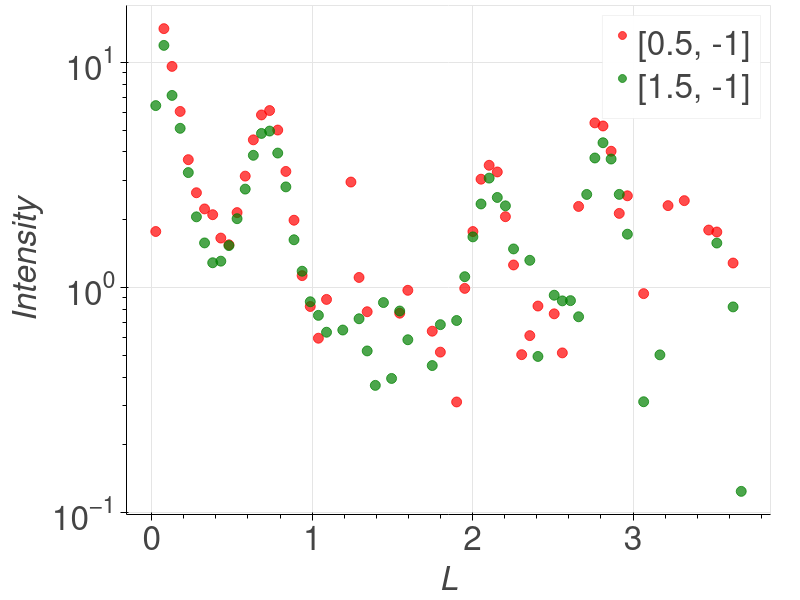
\includegraphics[width=0.95\textwidth]{Figures/sxrd_data/ctr/reconstruction_ctr_pt3o4.png}
        % 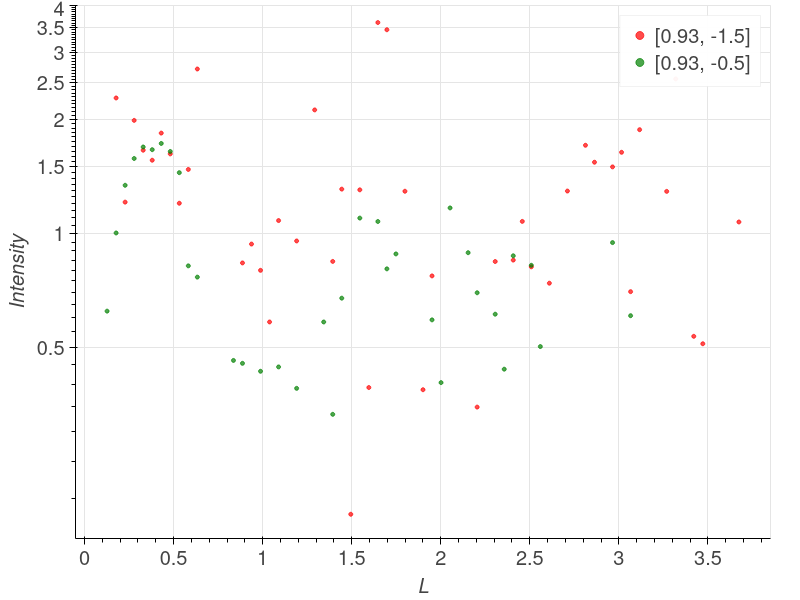
\includegraphics[width=\textwidth]{Figures/sxrd_data/ctr/reconstruction_ctr_pt3o4_no_data.png}
        \caption{CTR, peaks at L={0.7, 1.4, 2.1, 2.8} are characteristic of \ptthreeofour.}
        \label{fig:ctr_pt3o4}
    \end{figure}
    
    \column[T]{0.6\textwidth}
    
    \begin{figure}
        \centering
        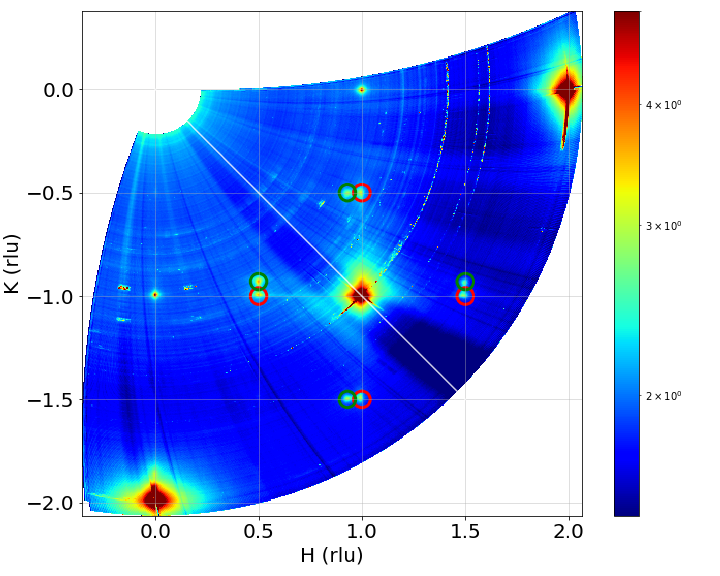
\includegraphics[trim=0 0 40 0, clip, width=0.95\textwidth]{Figures/sxrd_data/maps/Map_hkl_surf_or_1596-1635.png}
        \caption{Reciprocal space map with high oxygen atmosphere. The presence of oxygen induces two surface structures, \ptthreeofour and a slightly shifted \textcolor{green}{unknown structure} (no structure in L).}
        \label{fig:CondF1}
    \end{figure}

    \end{columns}

\end{frame}